
\documentclass[conference]{IEEEtran}
\IEEEoverridecommandlockouts
% The preceding line is only needed to identify funding in the first footnote. If that is unneeded, please comment it out.
\usepackage{cite}
\usepackage[utf8]{inputenc}
\usepackage{amsmath,amssymb,amsfonts}
\usepackage{algorithmic}
\usepackage{graphicx}
\usepackage{textcomp}
\usepackage{lipsum}
\usepackage{xcolor}
\usepackage{caption}
\usepackage{array}
\usepackage{siunitx}
\captionsetup[table]{name=Tabela}
\def\BibTeX{{\rm B\kern-.05em{\sc i\kern-.025em b}\kern-.08em
		T\kern-.1667em\lower.7ex\hbox{E}\kern-.125emX}}
\begin{document}
	
	\title{	Modelagem de um IP Soft Core utilizando Redes de Petri
	}
\author{\IEEEauthorblockN{1\textsuperscript{st} Pedro Lucas Falcão Lima}
	\IEEEauthorblockA{\textit{Departamento de Teleinformática (DETI)} \\
		\textit{Universidade Federal do Ceará (UFC)}\\
		Fortaleza, Brasil \\
		pedrolfalc@gmail.com}
	\and
	\IEEEauthorblockN{2\textsuperscript{nd} Giovanni Cordeiro Barroso}
	\IEEEauthorblockA{\textit{  Departamento de Teleinformática (DETI)} \\
		\textit{Universidade Federal do Ceará (UFC)}\\
		Fortaleza, Brasil \\
		gcb@fisica.ufc.br}
	
}
 	\maketitle
	
	\renewcommand{\abstractname}{Resumo}
	\begin{abstract}
		
		
			
	Sistemas de detecção de intrusão são cada vez mais necessários para garantir a segurança de serviços na internet, uma vez que as ameaças na rede vem desenvolvendo-se cada vez mais. Ataques do tipo DDoS são muito comuns atualmente, uma vez que já existem recursos suficientes para realizar esse tipo de ataque em tempo real. Apesar de existirem soluções em softwares para detectar ataques DDoS, muitas são ineficientes. Nesse trabalho foi modelado um soft ip core para ser implementado em  FPGAs que possuem capacidade de realizar a detecção de ataque DDoS em tempo real, em um tempo de menos de 1 \si{\micro}s. Além disso, o modelo desenvolvido objetiva baixa utilização de recursos, pois busca o mínimo uso de elementos. Por isso a modelagem foi feita utilizando Redes de Petri, que é uma ferramenta que possibilita a construção de modelos compactos e parametrizados. 
		
	\end{abstract}
	
	
	\renewcommand{\IEEEkeywordsname}{Palavras-chave}
	\begin{IEEEkeywords}
		Redes-em-Chip, falhas, tolerância, simulação, FPGA, desempenho, nuvem.
	\end{IEEEkeywords}
	
	\section{Introdução}
	
	
	Com a crescente difusão da internet e sistemas web na atualidade, cada vez mais
	serviços são disponibilizados por meio da rede mundial de computadores. Serviços tais como armazenamento, transações financeiras e plataformas de dados cadastrais são cada vez mais comuns. Por isso, é necessário que tais serviços cumpram os requisitos de disponibilidade e segurança. Assim, sistemas de detecção de intrusão (IDS), são comumente usados para garantir a segurança por meio de análise e detecção de tráfegos maliciosos,bem como tomar medidas corretivas em caso de tráfegos maliciosos.  \\ 
	Mediante a esse crescimento de usuários e serviços na internet, ameaças na rede vem
	desenvolvendo-se cada vez mais. Por isso, nota-se uma maior complexidade nessas ameaças.De acordo com \cite{b1} são considerados ataques a segurança quaisquer
	eventos que interrompam os procedimentos normais causando algum nível de crise, tais
	como invasões de computador, ataques de negação de serviço, furto de informações por
	pessoal interno. Ataques podem ser do tipo de negação de serviços. \\
	Os ataques DoS (sigla para Denial of Service), que podem ser interpretados como
	"Ataques de Negação de Serviços", consistem em tentativas de fazer com que computadores - servidores Web, por exemplo tenham dificuldade ou mesmo sejam impedidos de executar suas tarefas. Para isso, em vez de "invadir"o computador ou mesmo infectá-lo com malwares, o autor do ataque faz com que a máquina receba tantas requisições que esta chega ao ponto de não conseguir dar conta delas. Em outras palavras, o computador fica tão sobrecarregado que nega o serviço \cite{b2}. Ataques do tipo DoS distribuidos são chamados de ataques DDoS.\\ DDoS, sigla para Distributed Denial of Service, é um tipo de ataque DoS de grandes dimensões, ou seja, que utiliza até milhares de computadores para atacar uma determinada máquina, distribuindo a ação entre elas. Trata-se de uma forma que aparece constantemente no noticiário, já que é o tipo de ataque mais comum na internet \cite{b3}.\\ Para detectar ataques DDoS em tempo real, o mecanismo de detecção deve ser
	capaz de detectar ataques de forma eficiente de um pequeno conjunto de características relevantes. Portanto, é necessária uma medida efetiva para classificar um tráfego em tempo real.Essa detecção passa, por uma série de análises de dados, por isso é necessário a utilização de medidas estatísticas, consequentemente cálculos computacionalmente complexos. O alto rendimento é essencial para a escalabilidade da detecção , o que é necessário no caso de ataques DDoS.\\
	Diante disso, soluções baseadas em software são ineficientes para aplicações de
	tempo real, uma vez que eles exigem grande quantidade de ciclos de CPU de propósitos
	gerais. Logo, é necessário que soluções em hardware estejam presentes nas detecções de ataques DDoS . Podendo assim, ser gerados sistemas híbridos (hardware e software) que possuem alto desempenho e precisão.\\
	Por isso foi proposto um módulo de detecção , afim de 'garantir desempenho e
	precisão de ataques, utilizando FPGA(Field Programmable Gate Array), que junto a sistemas de softwares consigam detectar ataques DDoS. Para a construção e validação desse módulo foi realizado uma modelagem utilizando redes de petri, que é uma ferramenta que possibilita o desenvolvimento, simulação e avaliação de sistemas híbridos como os sistemas de tempo real.

	
	\section{Detalhamento Técnico}
A detecção de um ataque DDoS é um trabalho relativamente complexo, uma vez
que esse tipo de ataque ocorre em tempo real, e muitas vezes é difícil de ser identificado a máquina que é o atacante principal, por isso utilizamos o conceito de "tráfego não desejado". Como visto anteriormente, antes da ação do ataque acontecer, existem as ameaças aquela rede ou máquina, por isso tráfegos que não são desejados (que podem ser vistos como ameaça anteriormente a ação do ataque propriamente dito) devem ser identificados e o sistema de segurança podem tomar as devidas medidas. Existem muitas técnicas de detecção de ataques DDoS que fazem uso de cálculos estatísticos \cite{b4}, porém essas soluções não proporcionam alta precisão de detecção DDoS, pois fazem uso de apenas um pequeno conjunto de recursos de tráfego, ou seja, com poucos dados de tráfego a detecção se torna inviável. A Correlação é uma medida estatística que é muito utilizada nas detecções de ataques \cite{b5}.\\
Correlação é uma medida que mede o relacionamento entre duas variáveis . Uma
das maiores vantagens da correlação é que ela não necessita de uma grande quantidade de
variáveis, para chegar a uma conclusão de relacionamento entre dois conjuntos. Portanto
para uma detecção de ataques consistentes é necessária uma medida de correlação efetiva
para classificar ataques DDoS em tempo real, mesmo quando usa um pequeno número
de recursos de tráfego. Uma correlação de forma resumida, é um conjunto de cálculos
que, a partir das variáveis de entrada, retorna o relacionamento (similaridade, linearidade e direção) entre as variáveis, em um valor entre -1 e 1. Para calcular essa correlação, é necessário se ter os valores de entrada e um módulo (em hardware) que realize os cálculos, retornando o resultado da correlação, Para isso utilizamos a implementação de correlação em ataques DDoS proposto em \cite{b2}. As operações matemáticas necessárias para o calculo da correlação pode ser visto abaixo na figura \ref{ophw}.
	
	\begin{figure}[htbp]
		\centerline{\includegraphics[scale=1.0]{op2.jpg}}
		\caption{Operações de correlação em Hardware, em que x1,x2,x3,y1,y2 e y3 são valores de entrada e aT é o resultado da correlação}
		\label{ophw}
	\end{figure}
	
    Para realizar a computação dos cálculos da correlação é necessário da modelagem de pequenos módulos em RP, e que incluir num módulo de detecção de ataques. Este módulo de detecção em hardware é basicamente a implementação da formulação dos passos da correlação proposta. Para isso, é necessário adequar as operações para os componentes que estão disponíveis e foram escolhidos para realizar a computação de uma dada operação. Além disso, para otimizar o tempo de resposta é necessário uma organização dessas operações em ciclos de clock, para ter uma referência de tempo para cada computação realizada e assim organizar a sequência das operações.\\
	
	Com isso, a arquitetura de detecção de ataques é proposta com o nome de Nahid. Essa arquitetura possui componentes de diversos níveis,nos quais estão dispostos dependendo da operação que esteja sendo feita no momento, vale ressaltar que essas operações são aritméticas, mudança no tamanho da palavra, registro e seleção. Para o módulo de correlação em hardware receber as instâncias de tráfego no trabalho \cite{b2}, foi implementado um módulo chamado de pré-processador e ao final da computação, o módulo de hardware (Nahid) envia para outro módulo que irá realizar algum tratamento no sistema, chamado de gerenciador de segurança. Nota-se que os módulos do pré-processador e do gerenciador de segurança são
	implementados separadamente usando software. Essa modelagem pode ser vista na figura \ref{altonivel} 

	\begin{figure}[htbp]
	\centerline{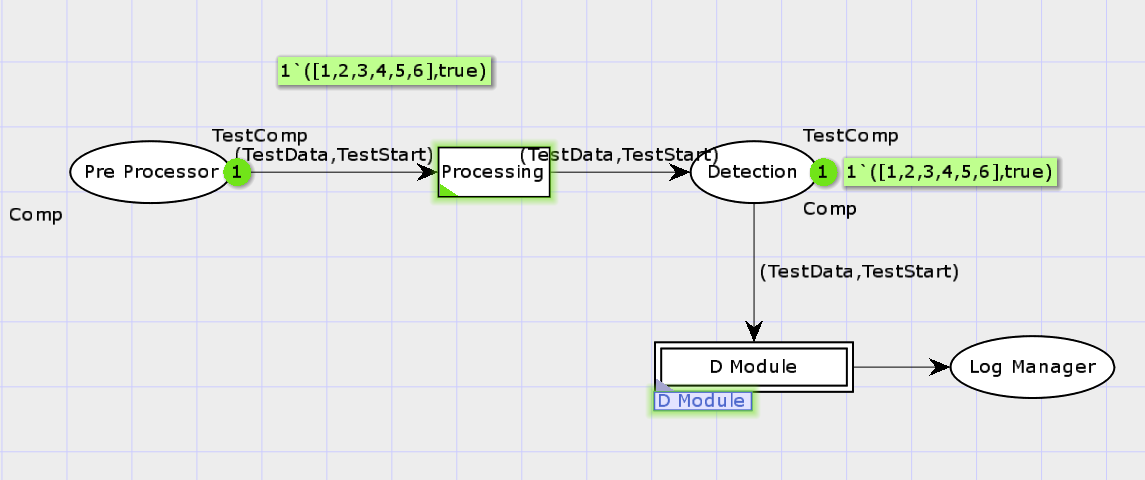
\includegraphics[scale=0.30]{an.png}}
	\caption{Sistema completo de detecção de ataques DDoS, modelado em redes de petri.}
	\label{altonivel}
	\end{figure}
	O "D Module"(Nahid) é o componente de mais alto nível, sendo ele quem recebe as entradas(perfil normal e instâncias de tráfego em análise) do módulo pré-processador e envia a saída\label{key}(resultado da análise) para o gerenciador de segurança. O Nahid é composto basicamente por dois componentes internos, são esses: Datapath e Controller. Além dos vetores de entrada citados anteriormente, o componente Nahid recebe os sinais de controle, clock e start (que são os sinais que indicaram o início da detecção e as mudanças de ciclos). Como foi projetado um módelo de um módulo de detecção o desenvolvimento dos sinais de clock foram realizados utilizando temporização nas RPs, então nesse caso não é uma entrada explicita no sistema. A modelagem do "D Module" pode ser vista na figura \ref{nahid} \\      
	
		\begin{figure}[htbp]
		\centerline{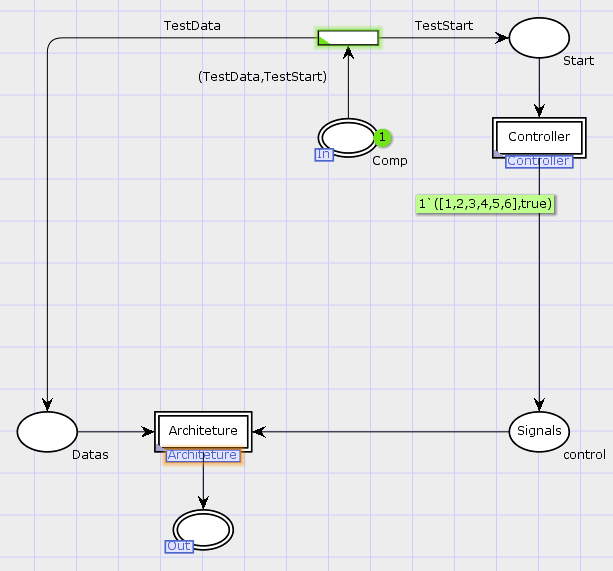
\includegraphics[scale=0.54]{nahid.png}}
		\caption{Componente Nahid: Módulo que recebe dados e calcula a correlação entre dois perfis, além de enviar para a saída do sistema completo. }
		\label{nahid}
	\end{figure}

O componente responsável por alocar todos os componentes que realizam as
operações da detecção é o Datapath. Por isso, o mesmo comporta no mínimo um dos
componentes de mais baixo nível, que serão descritos posteriormente. O Datapath recebe
os vetores de entradas(perfil normal e instâncias de tráfego em análise) do Nahid, pois esses
dados são selecionados, tratados e registrados pelos componentes internos do Datapath.
Porém para isso é necessário que seja indicado ao componente quais são as entradas a
serem processadas num dado ciclo, por isso o Datapath recebe como entrada seletores
provindos do Controller . Entretanto , o Datapath possui saídas para o controller, pois
em alguns ciclos é necessário de alguma confirmação de algum componente interno ao
Datapath, além disso a saída do sistema será um resultado registrado num componente
interno e será em enviado ao componente de mais alto nível (Nahid). A modelagem do Datapah pode ser visto na figura \ref{datapath}.

\begin{figure}[htbp]
	\centerline{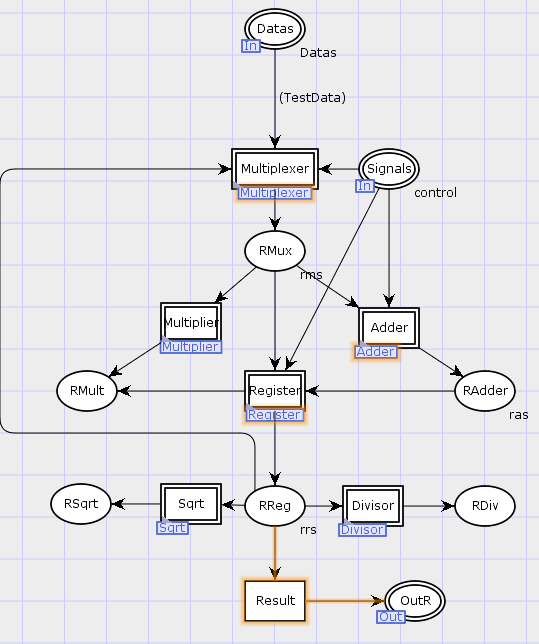
\includegraphics[scale=0.64]{datapath.png}}
	\caption{Componente Datapath: Módulo que aloca os componentes de mais baixo nível responsáveis por realizarem operações aritméticas.}
	\label{datapath}
\end{figure}
O componente responsável por organizar os ciclos das operações do Módulo Nahid
é o Controller. Quais componentes do Datapath que serão utilizados num determinado
ciclo de computação e em que ciclo teremos os resultados de uma dada operação, são as
principais funções desse componente. Esse componente, utiliza o conceito de máquina de
estados, para realizar uma computação cíclica e prática, afim dos cálculos serem realizados de forma otimizada. O Controller recebe o clk (clock do sistema) e o start (sinal que indica o início do módulo) do Nahid, para que o componente garante que o sistema está síncrono. Além dessas entradas, como dito anteriormente, recebe os sinais “valid out” dos componentes Divider e Sqrt. O Controller possui saídas para o Datapath, para indicar a esse componente o que será utilizado num dado ciclo.  A modelagem do Controller pode ser visto na figura \ref{controller}.
\begin{figure}[htbp]
	\centerline{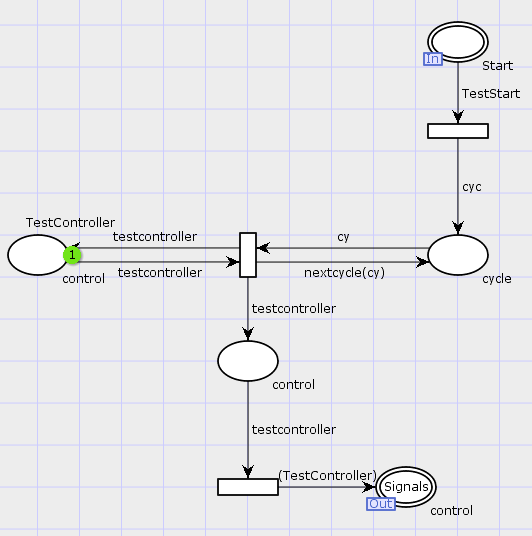
\includegraphics[scale=0.64]{controller.png}}
	\caption{Componente Datapath: Módulo que organiza a sequência das ações combinacionais do Nahid.}
	\label{controller}
\end{figure}

Com esses dois principais componentes Datapath e Controller pode-se realizar a modelagem de forma mais abstrata, porém houve uma maior dificuldade quanto ao tamanho da comunicação de dados uma vez que esse sistema possui 29 multiplexadores, 5 somadores, 5 multiplicadores, 11 registradores, 1 divisor e um componente que calcula raiz quadrada. Com a utilização de listas para realizar a a transferência de informação entre os componentes, a modelagem ficou complexa quanto à mudanças desses dados constantemente em uma linguagem funcional. Vale ressaltar que existem formas de simplificar mais ainda esse modelo que foi realizado, assim diminuindo consideravelmente essa complexidade. Uma medida adotada foi realizar um teste numa modelagem simples de  um ciclo (figura \ref{combinacional})  e assim construir o modelo posteriormente de forma incremental. 
\begin{figure}[htbp]
	\centerline{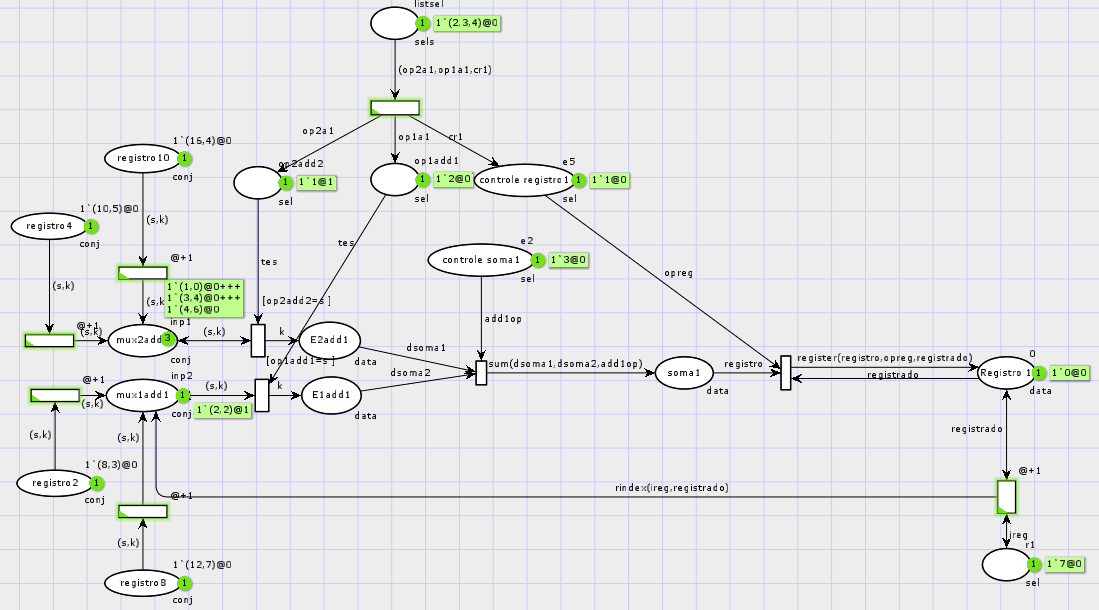
\includegraphics[scale=0.30]{Combinacional.png}}
	\caption{Modelo simplificado de um ciclo de computação}
	\label{combinacional}
Na figura \ref{combinacional} é mostrado alguns componentes básicos, como multiplexadores, somadores e registradores. Esses elementos também foram implementados utilizando RPs e as ferramentas em que os componentes de alto nível foram desenvolvidas, porém elas são facilmente simplificadas e destrinchadas no nível baixo do modelo hierárquico. Além disso, vale ressaltar que a modelagem desses componentes aritméticos é bem variável quanto a linguagens de descrição de hardware, por isso não vale a pena entrar mais fundo quanto a forma que está sendo realizada no modelo e sim ca influência de seu resultado mediante a uma latência de computação. 
\end{figure}

Esse modelo foi simulado e testado corretamente diversas vezes e com o teste de outros ciclos de computação, porém não foram realizado o uso de testes mais persistentes e com métricas reais, devido ao modelo ainda não possuir o módulo de detecção completo.
	\section{Resultados e Conclusões}
	
	Tendo em vista que a modelagem proposta inicialmente, requere uma certa complexidade de uso de listas e elementos indexadores, uma modelagem mais simples é uma solução significativamente mais mensurável para medir um dado modelo. Obtivemos resultados bem significantes quando implementamos esse modelo menor, e comprovamos a construção de módulos capazes de realizar as computações requeridas por essa correlação. Vale ressaltar, que para uma modelagem real e fiel a realidade é necessário um sistema completo, este deve possuir não só todos os módulos mas todas as sequências de computação. Por isso, é importante a construção desse módulo real a partir desse sistema simplificado. Além disso, após concluída essa fase de construção, deve ser realizado uma bateria de testes seguidas por simulações com métricas reais, para que assim novas otimizações possam ser realizadas numa nova modelagem, mais ainda, visualizamos oportunidade de redução do número de ciclos,através de uma paralelização ainda mais massiva das operações de cálculo do Nahid. Em outras palavras, para realizar teste de eficiências e mudanças de otimização é muito importante a modelagem feita e a forma em que é feita para assim a implementação desse e de outros sistemas de hardware.  
	
	
	\section*{Referências}
	\renewcommand{\section}[2]{}
	
	\begin{thebibliography}{00}
		\bibitem{b1}  PMANDIA, K.; PROSISE, C. Hackers resposta e contraataque. Rio de Janeiro: Campus,2001.
		\bibitem{b2}HOQUE, N. et al. Real-time DDoS Attack Detection Using FPGA. Computer Communications, v. 110, n. Supplement C, p. 48 – 58, 2017.
		nsactions on Electron Devices, vol. 47, no. 4, pp. 734-740, Apr 2000.
		
		\bibitem{b3}ALECRIM, E. Ataques DoS (Denial of Service) e DDoS (Distributed DoS).[S.l.]: Disponível na Internet em< http://www. infowester. com/col120904. php> em,2008.
		
		\bibitem{b4} AHMED, H. A. et al. Shifting-and-scaling correlation based biclustering algorithm.IEEE/ACM Transactions on Computational Biology and Bioinformatics,v. 11, n. 6, p. 1239–1252, Nov 2014.
		\bibitem{b5} YU, S. et al. Discriminating ddos attacks from flash crowds using flow correlation coefficient. IEEE Transactions on Parallel and Distributed Systems, IEEE, v. 23,n. 6, p. 1073–1080, 2012.
	
	\end{thebibliography}
	
	
\end{document}
